\chapter{图形摘要：用一张图表达研究贡献}

做遥感与深度学习交叉研究的博士生小周刚刚收到期刊的录用通知，编辑部在邮件里附了一条补充要求：一周内提交一张图形摘要（graphical abstract），随文章上线展示在期刊目录页与论文首页顶部。小周觉得这件事再简单不过——她打开论文源文件，找到精心绘制的 Figure 1（一张带跳跃连接、通道维数标注、多尺度注意力模块与损失函数公式的编码器—解码器网络结构图），等比例缩小后导出成图片交了上去。

两天后，技术编辑把这张图退了回来，退稿意见只有两句话：“这张图展示的是网络内部结构，不是你的研究贡献；而且缩到目录尺寸后，图里的文字完全看不清。”

许多作者第一次补交图形摘要时都踩过同一个坑：要么把论文里的网络框架图（Figure 1）直接缩小，要么把整篇论文的四五个实验结果面板硬塞进同一张画布，做成一张微型汇报海报。结果是熟悉这一小方向的同行不需要看它，跨方向的读者在期刊目录里扫一眼却既看不出论文要解决什么问题，也看不懂这项工作究竟发现了什么。本章专门解决这个任务：如何在严苛的尺寸与阅读时间约束下，用一张图准确、克制地表达一项研究的核心贡献与适用边界。

\section{图形摘要要回答什么}

图形摘要是放置在期刊在线目录（table of contents, TOC）、检索结果列表以及文章落地页顶部的单幅图件。它的核心使命非常单纯：让正在快速浏览目录或检索列表的读者在几秒钟内判断——\textbf{“这篇论文研究的问题和我有关吗？作者大致怎么做的？得到了什么有边界的结论？”}

要完成这个使命，一张合格的图形摘要只需要回答三个彼此咬合的问题：\textbf{研究问题（Question）—核心做法（Method）—主要发现与必要限定（Finding \& Limits）}。它不负责复述网络每一层的卷积核大小，不负责罗列超参数与消融实验，也不直接堆放带误差棒和显著性星号的原始数据图。

在动笔设计之前，必须先厘清图形摘要与另外三类常见学术图件的功能边界：

\begin{center}\footnotesize
\setlength{\tabcolsep}{3pt}
\renewcommand{\arraystretch}{1.15}
\begin{tabularx}{\linewidth}{@{}>{\raggedright\arraybackslash}p{22mm}>{\raggedright\arraybackslash}p{24mm}YY@{}}
\toprule
\textbf{图件类型} & \textbf{展示位置与停留时间} & \textbf{主要读者与核心任务} & \textbf{常见误用与禁忌} \\
\midrule
论文 Figure 1（方法或框架图） & 正文方法节内；读者结合正文阅读数分钟 & 已点进全文的小同行；交代模块连接、数据流向、张量维度或实验分组细节 & 直接缩小当图形摘要用，导致读者只看见网络结构，看不见研究问题与结果 \\
图形摘要（Graphical Abstract） & 期刊目录页、检索页与文章首页；停留约 $3\text{--}8$ 秒 & 跨方向浏览目录的同行；交代“问题—做法—发现与边界”，帮助判断是否读全文 & 塞入多面板数据图、参数表或微小图例，缩到目录尺寸后糊成一团 \\
视觉摘要（Visual Abstract） & 医学等期刊社交媒体账号与推文卡片；停留数秒 & 社交媒体上的研究者与临床医生；常采用固定分栏模板配关键指标，服务社交转发 & 把社交媒体的吸睛口号搬进期刊目录，或省略适用人群与条件限制 \\
学术海报（Poster） & 会议现场展板；驻足交谈 $2\text{--}5$ 分钟 & 会议参会者；完整呈现研究背景、方法框图、核心数据图与结论要点（见第 12 章） & 把海报的多栏排版直接压缩成图形摘要，字号缩小十倍后丧失可读性 \\
\bottomrule
\end{tabularx}
\end{center}

关于图形摘要能不能“提高引用率”，学术界做过实证比较，结论并不一致。Pferschy-Wenzig 等人（2016）对比了发表在 \textit{Molecules} 期刊上带图形摘要与不带图形摘要的论文，发现在该研究所考察的样本与时间窗口内，带图形摘要的文章在引用次数、摘要浏览量和全文下载量上并未表现出更高的数值（具体样本构成与分析方法建议读者阅读原文）。另一方面，Ibrahim 等人（2017）针对外科学论文在社交媒体传播开展的前瞻性病例对照交叉研究显示，附带视觉摘要的推文在曝光量、转发数和文章访问量上高于纯文字推文。

这两项针对不同传播场景的研究提醒我们：\textbf{不要承诺或指望“画了图形摘要就会涨引用”，更不能为了博眼球而夸大结论。}图形摘要真正的价值在于\textbf{准确的快速理解}——在几秒钟内帮合适的读者认出你的工作，同时如实划定结论成立的前提，不让读者产生“这篇论文已经彻底解决某问题”的误判。

\section{先读期刊要求：比例先于构图}

许多研究者习惯先画好一张满意的图，等到投稿系统上传文件时才去查期刊指南，结果发现画布比例完全不对：原本按正方形排好的环绕式构图，硬塞进 $5:2$ 的横幅框里，要么左右两侧留下大片空白，要么上下被裁切、元素被迫压扁重排。

在图形摘要的制作流程里，\textbf{期刊格式要求不是最后一步的“导出设置”，而是第一步的“构图约束”}。不同出版社对图形摘要（或目录图 TOC graphic）的画布长宽比、最小像素、字体字号和内容禁区有着截然不同的规定。表~\ref{tab:ch10-01-rules} 与图~\ref{fig:ch10-01} 汇总了三家代表性出版社（Elsevier、Cell Press 与 ACS）的典型规范。

\begin{table}[htbp]\centering\footnotesize
\setlength{\tabcolsep}{3pt}
\renewcommand{\arraystretch}{1.15}
\caption{三类代表性出版社的图形摘要/目录图规范对比（2026 年 10 月访问官方页面整理；同一出版社不同期刊可能另有规定，投稿前务必以目标期刊当前页面为准）。}\label{tab:ch10-01-rules}
\begin{tabularx}{\linewidth}{@{}>{\raggedright\arraybackslash}p{22mm}>{\raggedright\arraybackslash}p{28mm}>{\raggedright\arraybackslash}p{26mm}Y@{}}
\toprule
\textbf{出版社 / 代表刊} & \textbf{尺寸与长宽比} & \textbf{分辨率、字体与格式} & \textbf{核心内容与版式规则} \\
\midrule
Elsevier（通用指南） & 最小 $1328 \times 531\ \text{px}$（宽 $\times$ 高）；更大尺寸保持 $500:200$（即 $5:2$）横幅比例 & $\ge 300\ \text{dpi}$；Times、Arial、Courier 或 Symbol；字号须足够大以适应约 $200\ \text{px}$ 高的目录窗口；支持 TIFF、EPS、PDF、MS Office & 有清楚的起点和终点，宜从左到右或从上到下阅读；减少干扰元素；文字必须在图像文件内，图外不另附文字或提要；不要多余留白，不在图内写“Graphical Abstract”标题 \\
Cell Press（官方博客与 \textit{Cell Reports} 清单） & 单面板正方形，$1200 \times 1200\ \text{px}$（各边相等；非正方形上线时画布可能被扩展） & $300\ \text{dpi}$；Arial 字体 $12\text{--}16\ \text{pt}$（更小字号在网上不可读）；支持 TIFF、PDF、JPG，不接受 PowerPoint & 单面板构图；指南建议用简洁视觉概念传达核心要点，不包含数据类元素（各子刊核对表数字可能不同，以目标刊当前页面为准） \\
ACS（以 \textit{J. Org. Chem.} 与 \textit{Langmuir} 为例） & 目录/摘要图物理尺寸不大于 $8.25 \times 4.45\ \text{cm}$（$3.25 \times 1.75\ \text{in}$，按 $300\ \text{dpi}$ 折算约 $975 \times 526\ \text{px}$） & 依各刊附录要求；通用图形指南建议无衬线字体（如 Arial 或 Helvetica） & 与标题一起给出文章要点的快速视觉印象；原创、无版权元素、不与正文图重复；\textit{J. Org. Chem.} 要求避免出现真实人物形象 \\
\bottomrule
\end{tabularx}
\end{table}

把这三类画布按同一比例尺画在同一张图上（图~\ref{fig:ch10-01}），就能直观看出为什么“比例决定构图，缩略图决定字号”。

\begin{figure}[htbp]\centering
\resizebox{\linewidth}{!}{% FIG ch10-01 ga-formats (Chinese)
\usetikzlibrary{positioning}
\begin{tikzpicture}[x=0.06mm,y=0.06mm, font=\sffamily\small, text=BookInk]
  \tikzset{
    frame/.style={draw=BookInk, line width=0.35mm, fill=white},
    guide/.style={draw=BookInk!30, line width=0.25mm},
    figcap/.style={font=\sffamily\small, text=BookInk, align=center},
  }
  % Bottom-align three canvases (Cell is tallest: 1200 px).
  \def\baseY{1200}
  % Elsevier 1328 x 531
  \draw[frame] (0,\baseY-531) rectangle (1328,\baseY);
  \node[figcap, anchor=south] at (664,\baseY-531-18) {Elsevier 通用指南};
  \node[figcap, font=\scriptsize, text=BookInk!85] at (664,\baseY-531-38)
    {$\geq 1328 \times 531$ px（5:2）};
  \draw[guide, -{Stealth[length=2mm]}] (120, \baseY-265) -- (1208, \baseY-265);
  % TOC thumbnail 500 x 200 (5:2 at 200 px high)
  \draw[frame] (40, \baseY-531-280) rectangle (540, \baseY-531-80);
  \node[figcap, font=\scriptsize] at (290, \baseY-531-300) {目录中的显示尺寸（约 200 px 高）};
  \draw[guide, thin] (664, \baseY-531) -- (290, \baseY-531-80);
  % Cell Press 1200 square
  \draw[frame] (1450, 0) rectangle (2650, 1200);
  \node[figcap, anchor=south] at (2050, -18) {Cell Press};
  \node[figcap, font=\scriptsize, text=BookInk!85] at (2050, -38)
    {$1200 \times 1200$ px，300 dpi};
  \draw[guide] (2050, 600) -- (1750, 900);
  \draw[guide] (2050, 600) -- (2350, 900);
  \draw[guide] (2050, 600) -- (2350, 300);
  \draw[guide] (2050, 600) -- (1750, 300);
  \draw[guide, -{Stealth[length=1.8mm]}] (1750, 900) -- (2350, 300);
  % ACS 975 x 526 (300 dpi from cm)
  \draw[frame] (2780, \baseY-526) rectangle (3755, \baseY);
  \coordinate (acs-cap) at (3267.5, \baseY-526);
  \node[figcap, anchor=north, text width=50mm, align=center] (acs-t) at ([yshift=-1.5mm]acs-cap)
    {ACS（以 \textit{J. Org. Chem.} 为例）};
  \node[figcap, font=\scriptsize, text=BookInk!85, anchor=north, text width=50mm, align=center,
    below=2.5mm of acs-t] (acs-m)
    {$\leq 8.25 \times 4.45\ \mathrm{cm}$};
  \node[figcap, font=\scriptsize, text=BookInk!85, anchor=north, text width=50mm, align=center,
    below=1.5mm of acs-m]
    {像素按 300 dpi 换算：$975 \times 526$ px};
  \draw[guide, -{Stealth[length=2mm]}] (2880, \baseY-263) -- (3655, \baseY-263);
  \node[figcap, font=\scriptsize, text=BookInk!70, anchor=north west] at (0, -75)
    {以目标期刊当前页面为准（2026 年 10 月访问）};
\end{tikzpicture}
}
\caption{三类图形摘要/目录图要求的形状与尺度对比（按同一比例绘制）。数值摘自 Elsevier 通用指南、Cell Press 官方说明与 ACS \textit{J. Org. Chem.} 作者指南（2026 年 10 月访问）；同一出版社的不同期刊可能另有规定，投稿前请以目标期刊当前页面为准。ACS 要求为物理尺寸，像素按 $300\ \text{dpi}$ 换算仅供比较。}\label{fig:ch10-01}
\end{figure}

观察图~\ref{fig:ch10-01} 可以得出三条直接指导作图的硬约束：

第一，\textbf{长宽比锁定阅读路径的走向}。Elsevier 的 $5:2$ 画布是宽扁横幅，适合“从左到右”分三到四段平铺叙事；Cell Press 的 $1200 \times 1200\ \text{px}$ 画布是正方形，若只把三四个小图标横排在中间，上下就会空出大片白底，因此更适合“中心图加四周环绕”或上下两行折返（Z 字形）构图；ACS 的目录图物理面积小（宽仅 $8.25\ \text{cm}$），能容纳的视觉节点更少。

第二，\textbf{目录缩略图高度决定最小字号与元素数量}。图~\ref{fig:ch10-01} 左下角的小框标出了 Elsevier 指南专门强调的一项约束：在线目录中，图形摘要会被缩小到\textbf{约 $200\ \text{px}$ 高}的窗口中显示（按 $5:2$ 比例即 $500 \times 200\ \text{px}$）。哪怕原图画在 $2000 \times 800\ \text{px}$ 的高清画布上，到了目录页高度也会缩为四分之一。原图上 $14\ \text{px}$ 高的小字缩后只剩 $3.5\ \text{px}$，完全无法辨认。

第三，\textbf{投稿前以目标期刊当前页面为准并记录访问日期}。同一出版社旗下不同子刊的核对表可能存在差异，且规则会随时间调整。动笔前应先打开目标期刊当前的作者指南页，把网址、访问日期、比例、像素、字体和格式要求记入图片档案。本章主案例设想投稿至采用 Elsevier 通用指南的遥感类期刊，统一按 **$5:2$ 横幅、导出尺寸 $2000 \times 800\ \text{px}$（满足 $\ge 1328 \times 531\ \text{px}$）、目录缩略图高 $200\ \text{px}$** 设计与核验。

\section{从论文到四行贡献卡}

确定画布规格后，下一步不是立刻打开生成工具写提示词，而是先把论文浓缩成一张四行\textbf{“贡献卡”（contribution card）}。

\begin{BookNote}
\textbf{说明：}下面的研究是为本章虚构的教学情境，方法与结论均按领域常识保守设定，不对应任何已发表论文的结果。
\end{BookNote}

我们先交代本章主案例的学科背景。火灾发生后，灾后评估需要绘制\textbf{过火区（burned area）}范围，即标出已经被火烧过的地表。植被烧毁后，近红外（NIR）反射率下降、短波红外（SWIR）反射率上升，因此归一化燃烧比 $\text{NBR} = (\text{NIR} - \text{SWIR}) / (\text{NIR} + \text{SWIR})$ 在火前与火后的差值（$\text{dNBR}$）配合固定阈值，是提取过火区的常用基线（Chuvieco 等，2019；Roy 等，2019）。广泛使用的全球中分辨率过火区产品（如 MODIS MCD64A1）按月发布，分辨率约 $500\ \text{m}$（Giglio 等，2018）；更高分辨率的 Landsat 与 Sentinel-2 能刻画更细的火场边界（Roy 等，2019），深度学习语义分割网络也已被用于 Sentinel-2 过火区制图（Knopp 等，2020）。

围绕这一背景，小周所在课题组撰写了如下教学论文摘要：

\begin{Prompt}
Fictional teaching manuscript for Chapter 10 — not a real study.
Title: Earlier burned-area mapping from Sentinel-2 image pairs with a
segmentation network
Abstract. Burned-area information supports post-fire assessment, but widely
used moderate-resolution products are released monthly. We ask whether burned
area can be mapped as soon as the first cloud-free post-fire Sentinel-2 image
becomes available. We train an encoder-decoder segmentation network on
co-registered pre-fire and post-fire image pairs, using near-infrared and
shortwave-infrared bands, to predict a per-pixel burned probability. On
held-out fire events, the network's maps agree more closely with reference fire
perimeters than a fixed-threshold dNBR baseline, especially along fragmented
edges and in mixed vegetation. Agreement decreases when clouds or smoke obscure
the post-fire scene and in ecoregions that differ from the training data. The
approach maps areas that have already burned; it does not detect active fires
or forecast fire occurrence. Its timeliness is bounded by satellite revisit and
cloud-free acquisitions. We discuss how reference-perimeter uncertainty and
geographic transfer should be evaluated before operational use.
\end{Prompt}

为了防止把波段列表、配准细节和次要讨论统统塞进图形摘要，我们用一张\textbf{四行贡献卡}来强制做减法。卡片只写四行：\textbf{问题、方法、发现、限定条件}，遵循三条筛选规则：
\begin{enumerate}
\item \textbf{每行只写一句话、一个主语：}剥离属于正文方法节的技术参数（波段编号、损失函数、训练超参数）。
\item \textbf{“发现”严格保持论文中的措辞强度：}论文证明的是“比固定阈值 dNBR 基线更接近参考边界”，就绝不升级成“解决了复杂地形过火区制图难题”。
\item \textbf{“限定条件”选一条“删掉就会让读者误解结论”的边界：}本案例必须随结论一起交代两点——一是**绘制的是已过火区域，不是活跃火点探测（常靠热红外传感器）或火灾预测**；二是**依赖无云观测，时效受卫星重访周期（数天量级）和云、烟遮挡限制**。
\end{enumerate}

从上述摘要提炼出的作者确认版贡献卡见表~\ref{tab:ch10-02-card}。

\begin{table}[htbp]\centering\footnotesize
\setlength{\tabcolsep}{3pt}
\renewcommand{\arraystretch}{1.15}
\caption{从教学案例摘要提炼的四行贡献卡（作者确认版）。}\label{tab:ch10-02-card}
\begin{tabularx}{\linewidth}{@{}>{\raggedright\arraybackslash}p{12mm}Y>{\raggedright\arraybackslash}p{32mm}>{\raggedright\arraybackslash}p{34mm}@{}}
\toprule
\textbf{行} & \textbf{贡献卡内容（中文）} & \textbf{来自摘要哪一句} & \textbf{主动删去了什么及原因} \\
\midrule
问题 & 能否在火后第一景无云影像到达后，就绘制出过火区？ & ``We ask whether burned area can be mapped as soon as the first cloud-free post-fire Sentinel-2 image becomes available.'' & 月度产品的分辨率背景与灾后评估用途（留给引言） \\
方法 & 用火前/火后 Sentinel-2 影像对训练分割网络，输出逐像元过火概率 & ``We train an encoder-decoder segmentation network on co-registered pre-fire and post-fire image pairs...'' & 近红外/短波红外波段列表、配准细节与网络层数（属于方法细节） \\
发现 & 在留出测试火场上，比固定阈值 dNBR 基线更接近参考边界，尤其在破碎边界处 & ``On held-out fire events, the network's maps agree more closely with reference fire perimeters than a fixed-threshold dNBR baseline...'' & 具体指标数值（本教学情境不设数字，只表达边界贴合对比） \\
限定 & 绘制的是已过火区域，不是火点探测或火灾预测；受云、烟和重访周期限制 & ``The approach maps areas that have already burned; it does not detect active fires or forecast fire occurrence. Its timeliness is bounded by...'' & 跨生态区泛化与参考边界误差（放在图注与正文） \\
\bottomrule
\end{tabularx}
\end{table}

把四行连成一句话贡献：\textbf{一景无云影像就能出过火区图，比阈值法更贴近真实边界——但它画的是已经烧过的地方，而且要等到天晴。}

接着把以下任务书保存在自己的文档里，在 \scidraw{} 的\textbf{科研绘图向导}（\sdtool{figure-workflow}）中选“图形摘要”，从第 1 步“生成初稿”进入图形摘要生成器（\sdtool{graphical-abstract-maker}）粘贴使用（向导只组织步骤，不检查科学内容；完整版本见本书仓库 \texttt{cases/} 目录）：

\begin{Prompt}
【用途与读者】Elsevier 遥感类期刊图形摘要；读者为遥感与生态研究者，多不熟悉深度学习细节。
【尺寸】横幅 5:2，导出 2000 x 800 px（>= 1328 x 531 px），目录缩至约 200 px 高。
【目标】5 秒看懂：火后第一景无云影像 -> 分割网络 -> 过火区图，比阈值法更贴近参考边界；同时看到“已过火区制图、非火点探测、受云烟限制”。
【材料】作者确认的四行贡献卡与论文摘要；图中不出现论文以外的主张。
【对象】(1) 火前/火后扁平示意影像图块（非照片、非真实影像）；(2) 编码—解码沙漏形网络图标（不画层数）；(3) 输出过火区多边形图块；(4) 对比小插图：参考边界（深灰实线）、模型（蓝实线）与阈值法（浅灰虚线）；(5) 限定图标：灰云遮挡的影像小图块。
【关系】影像对 -> 网络 -> 过火区图（两支同型箭头）；对比插图置于右侧不画箭头；云图标靠近输入端。
【布局】左->右叙事四段；顶部 15% 留给标题句，底部 12% 留给限定短句。
【视觉】白底，扁平二维矢量风格；未过火植被低饱和绿，过火区暖棕橙，网络蓝灰，全图不超 3 个色相加灰。
【文字】底图不含任何文字；文字在 LaTeX/TikZ 中叠加，英文不超 35 词（中文不超 60 字）。
【限制】不画火焰、烟柱、地球、写实卫星、时钟、警报、数字、坐标轴；不用“预测”“实时”“全球”。
【验收】贡献卡四行均在图中；无超范围元素；缩到 200 px 高阶段名可读；底图无字；比例 5:2。
\end{Prompt}

注意任务书的一条关键决定：所有“影像”均画成\textbf{扁平示意图块}，并在说明中注明“示意，非真实影像”。如果让图像模型画出照片质感的卫星图，读者就会把它当成真实观测证据；若确需展示真实影像，必须使用论文自有数据或公有领域影像（如 USGS Landsat）并写明来源与处理。

\section{用 SciDraw AI 把 PDF 变成候选提示词}

进入 \scidraw{} 的图形摘要工具（\sdtool{graphical-abstract-maker}）时，可以上传论文 PDF 让系统自动生成一段视觉提示词。要正确使用它，必须先清楚它的读取边界（图~\ref{fig:ch10-02}）。

\begin{figure}[htbp]\centering
\resizebox{\linewidth}{!}{% FIG ch10-02 paper-to-card (Chinese)
\usetikzlibrary{arrows.meta,calc,fit,positioning}
\begin{tikzpicture}[
  font=\sffamily\footnotesize,
  node distance=4mm and 6mm,
  box/.style={
    draw=BookRule, line width=0.4pt, rounded corners=2pt,
    align=center, inner sep=5pt, text=BookInk, text width=22mm,
  },
  autobox/.style={box, dashed, fill=BookPale!40},
  authorbox/.style={box, fill=white},
  limitbox/.style={authorbox, draw=BookTeal, line width=0.9pt},
  flow/.style={-{Stealth[length=2mm]}, draw=BookInk!55, thin},
  note/.style={font=\scriptsize, text=BookInk!75, align=left},
]
  \node[authorbox, minimum width=24mm, minimum height=28mm] (pdf) {%
    \textbf{论文 PDF}\\[2pt]
    \tikz{\draw[fill=BookPale!50, draw=BookInk!30] (0,0) rectangle (1.4,1.8);
      \draw[fill=BookTeal!25, draw=BookTeal!60] (0,0.9) rectangle (1.4,1.8);
      \node[font=\tiny, anchor=west] at (1.55,1.35) {前 5 页};
      \node[font=\tiny, anchor=west] at (1.55,0.45) {其余页};}};
  \node[autobox, right=of pdf] (auto) {PDF\\转提示词};
  \node[autobox, right=of auto, text width=28mm] (prompt) {60--110 词的\\视觉提示词};
  \node[authorbox, below=10mm of pdf, text width=26mm] (full) {通读\\整篇论文};
  \node[authorbox, right=of full, text width=30mm] (card) {%
    贡献卡四行\\[1pt]
    \begin{tabular}{@{}c@{}}
      问题\\方法\\发现\\\textbf{限定}
    \end{tabular}};
  \node[limitbox, fit=(card), inner sep=1pt] {};
  \node[authorbox, right=12mm of prompt, text width=32mm] (merge) {逐行比对：\\补回限定条件、\\删去超出论文的说法};
  \node[authorbox, right=of merge, text width=28mm] (final) {作者确认的\\生成提示词};
  \draw[flow] (pdf) -- (auto);
  \draw[flow] (auto) -- (prompt);
  \draw[flow] (full) -- (card);
  \draw[flow] (prompt.east) -| (merge.west);
  \draw[flow] (card.east) -| (merge.south);
  \draw[flow] (merge) -- (final);
  \node[note, anchor=north west] at (pdf.south west) {约 6{,}000 字符上限};
  \node[note, anchor=north] at ($(auto)!0.5!(prompt)+(0,-8mm)$) {自动路径（虚线框）};
  \node[note, anchor=north] at ($(full)!0.5!(card)+(0,-8mm)$) {作者路径（实线框）};
  \node[note, anchor=north east] at (final.south east) {向导与工具不检查科学内容};
\end{tikzpicture}
}
\caption{从论文到图形摘要提示词的两条路径。\scidraw{} 的图形摘要入口只读取 PDF 前 5 页、最多约 $6{,}000$ 个字符，并生成一段简短的视觉提示词；它不理解整篇论文。作者的贡献卡来自全文，二者逐行比对后才形成生成提示词，限定条件尤其需要作者补回。}\label{fig:ch10-02}
\end{figure}

如图~\ref{fig:ch10-02} 所示，上传 PDF（上限 $20\ \text{MB}$）后，系统的实际行为有三项硬约束：
\begin{enumerate}
\item \textbf{只读前 5 页、最多保留约 $6{,}000$ 字符：}系统并非理解整篇论文。常规投稿手稿的前 5 页往往只到引言，后文的实验退化条件与讨论节局限性根本不在读取范围内。
\item \textbf{压缩为 $60\text{--}110$ 词的视觉提示词：}系统内部指令要求省略文献引用、$p$ 值、无依据主张和次要方法细节，聚焦于核心问题、方法与发现的视觉画面。
\item \textbf{限定条件常被当作“次要细节”省掉：}由于指令倾向于组织积极、简洁的视觉主干，“不探测活跃火点”“受云烟和重访限制”这类否定性边界极易在压缩中丢失，有时还会混入“实时”“预警”等加强词。
\end{enumerate}

因此，应当把自动生成的提示词当作\textbf{“第二位只读了论文开头的读者画的速写”}。实操时遵循三步核对法：第一，上传 PDF 后将返回的提示词原文連同读取范围记录存档；第二，对照作者贡献卡逐行核对（表~\ref{tab:ch10-03-compare}）；第三，补回限定条件、删去超出论文的说法，再生成候选图。

\begin{table}[htbp]\centering\footnotesize
\setlength{\tabcolsep}{3pt}
\renewcommand{\arraystretch}{1.15}
\caption{使用 PDF 转提示词入口时的逐行核对清单（对照作者贡献卡四行检查什么与如何修正）。}\label{tab:ch10-03-compare}
\begin{tabularx}{\linewidth}{@{}>{\raggedright\arraybackslash}p{14mm}>{\raggedright\arraybackslash}p{32mm}YY@{}}
\toprule
\textbf{贡献卡行} & \textbf{作者贡献卡基准} & \textbf{检查自动生成的 60--110 词提示词时要核对什么} & \textbf{作者修正与补回动作} \\
\midrule
问题 & 火后第一景无云影像到达后能否绘制过火区 & 是否把“第一景无云影像”改写成了“实时（real-time）”或“早期预警”；是否要求画正在燃烧的火焰 & 删去“实时/预警”字眼与火焰元素；明确起点是火前与火后两块静态示意地块 \\
方法 & 火前/火后 Sentinel-2 影像对输入分割网络 & 是否要求画复杂三维卷积层、发光大脑或写实卫星；是否混入正文未用的传感器 & 固定为“两块并排方形示意图块 + 一个简洁的蓝灰色沙漏形编码—解码图标” \\
发现 & 在测试火场上比固定阈值 dNBR 基线更贴近参考边界 & 是否只画输出图而漏掉与阈值法基线及参考边界的对比；或要求画柱状图和百分比数字 & 补入第四阶段“同一地块三条边界线（参考深灰实线、模型蓝实线、阈值法浅灰虚线）对比插图”，禁画数字 \\
限定 & 已过火区域制图（非火点探测/预测）；受云、烟和重访限制 & 重点查提示词里有无表达“需无云观测”的视觉元素，以及是否预留了叠加限定句的空白带 & 在输入端补回“被灰云部分遮挡的小图块”，并要求顶部 $15\%$ 与底部 $12\%$ 留白 \\
\bottomrule
\end{tabularx}
\end{table}

经逐行核对并补回限定条件后，整理出供图形摘要或绘图入口使用的中文生成提示词：

\begin{Prompt}
图形摘要，横幅 5:2，白底，扁平二维矢量风格，无渐变、无阴影、无 3D。
图中不要出现任何文字、字母或数字，文字之后由作者添加。
从左到右四段：
(1) 两块并排的方形影像图块（火前：低饱和绿色植被斑块；火后：同一地块，中间有一片暖棕橙色区域），上方一块带一小朵灰云的影像图块，略小，放在输入区角落；
(2) 一个蓝灰色的沙漏形网络图标（编码—解码），不画神经元层；
(3) 同一地块的输出图：暖棕橙色过火区多边形，边缘清晰；
(4) 一个小的对比插图：同一地块轮廓上，深灰实线为参考边界，蓝色实线紧贴它，浅灰虚线明显偏离。
两支同样的深灰流程箭头连接 (1)->(2)、(2)->(3)，(3) 与 (4) 之间不画箭头。
顶部 15% 与底部 12% 留白。颜色只用低饱和绿、暖棕橙、蓝灰与灰。
不要火焰、烟、地球、卫星写实模型、时钟、警报、图表、坐标轴。
\end{Prompt}

\section{两种构图候选：叙事式与中心图式}

很多作者点选“一次生成 4 张候选图”就以为完成了构图比选。其实，\textbf{共享同一段提示词批量生成的图片，只是同一布局的随机变体}，并不等于两种有理由的构图。真正的构图比选需要作者在提示词里分别写明不同的空间结构。本节对比图形摘要最常用的两种构图：\textbf{左$\rightarrow$右叙事式（候选 A）}与\textbf{中心图式（候选 B）}。

\textbf{构图候选 A（左$\rightarrow$右叙事式）}将“输入 $\rightarrow$ 模型 $\rightarrow$ 输出 $\rightarrow$ 发现”平铺为横向四段。提交的英文提示词关键部分如下（完整版本见本书仓库 \texttt{cases/} 目录）：

\begin{Prompt}
Graphical abstract base art, wide banner, aspect ratio 5:2 (2000 x 800 px),
pure white background, flat 2D vector illustration, flat fills, thin dark gray
outlines, no gradients, no shadows, no 3D, no photographic texture.
ABSOLUTELY NO TEXT: no letters, no words, no numbers, no symbols, no labels.
Keep the top 15% and the bottom 12% of the image completely empty.
Four equal-width stages from left to right, vertically centered:
1. Input (x 0.04-0.25): two square map tiles side by side (left: muted green
   vegetation with a thin pale-blue river line; right: same patch and river with
   an irregular warm brown-orange burned area). Above them, smaller, a third
   square tile partly covered by a flat light-gray cloud shape.
2. Model (x 0.30-0.46): a single blue-gray hourglass shape of stacked rounded
   rectangles that narrow to a waist and widen again (encoder-decoder).
3. Output (x 0.52-0.72): one square map tile of the same patch in very pale gray
   with a crisp warm brown-orange burned-area polygon.
4. Comparison (x 0.77-0.96): a small square inset showing three boundary lines:
   dark gray solid (reference), blue solid closely following it, light gray
   dashed clearly deviating from it.
Two identical dark gray arrows connect stage 1 to 2 and 2 to 3; no arrow between
3 and 4. Do not draw: flames, smoke, globes, satellites, clocks, alarms, charts.
\end{Prompt}

我们将该提示词生成了两次，选定第一次生成图作为候选 A 底图，并在 LaTeX 中叠加阶段编号用于构图讲评（图~\ref{fig:ch10-03}）。

\begin{figure}[htbp]\centering
\begin{tikzpicture}
\node[anchor=south west,inner sep=0] (img) at (0,0) {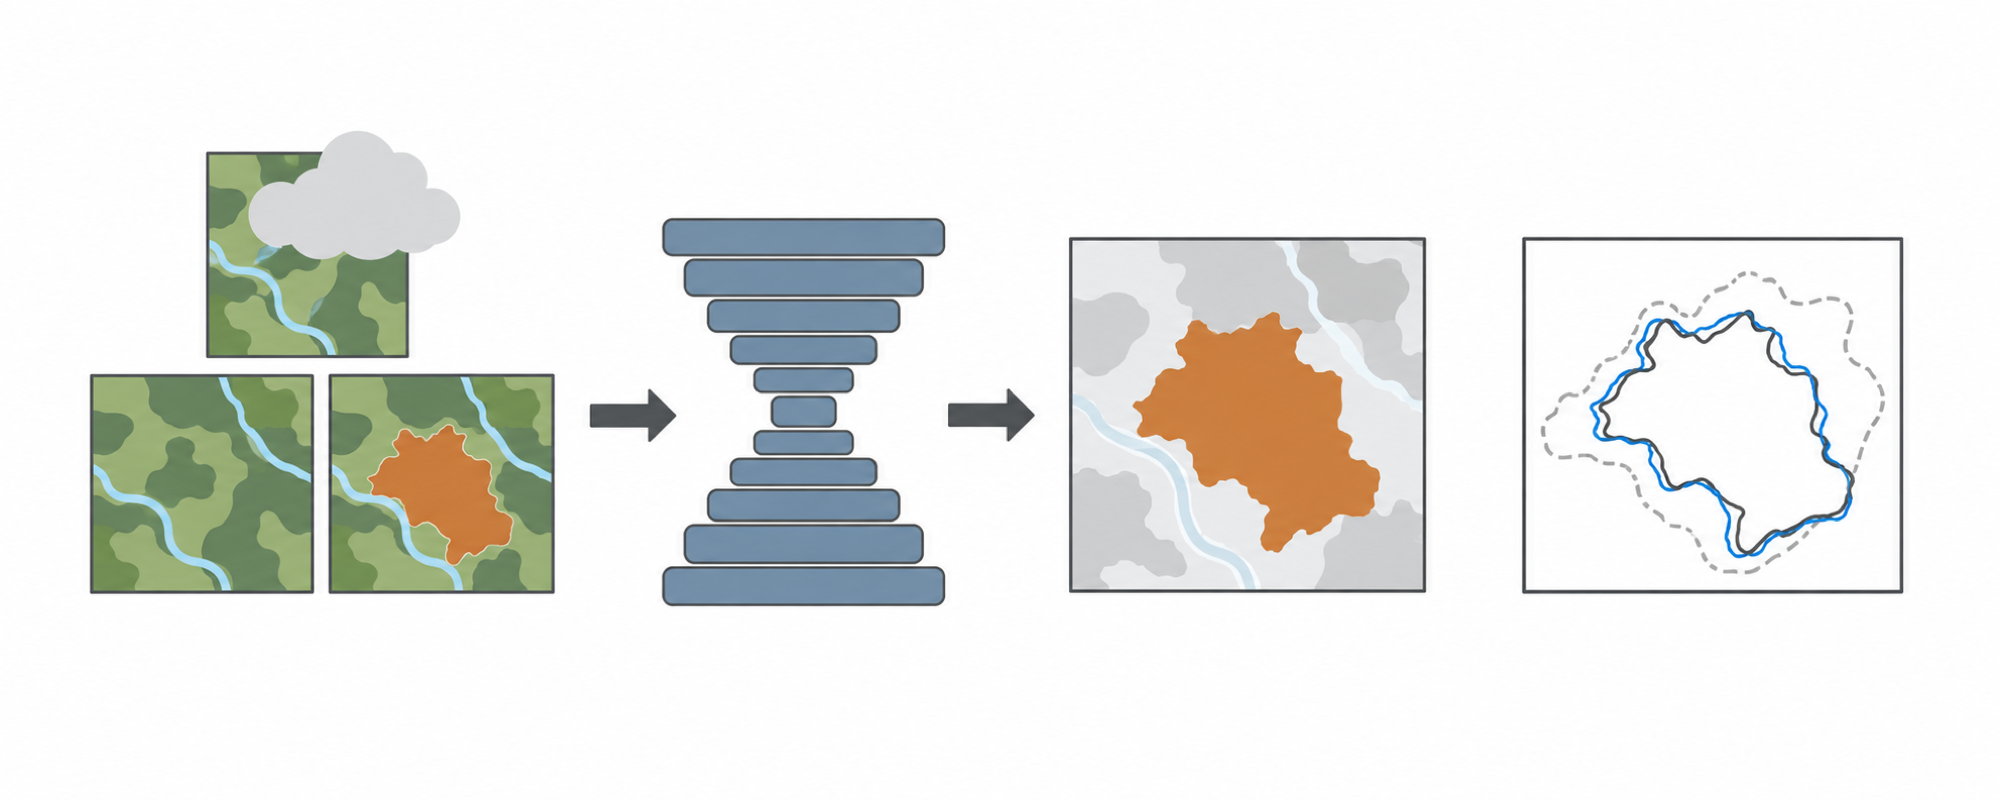
\includegraphics[width=\linewidth]{figures/ch10/ch10-03-composition-a-narrative.png}};
\begin{scope}[x={(img.south east)},y={(img.north west)}]
  \tikzset{stglbl/.style={font=\sffamily\footnotesize\bfseries,text=BookInk,fill=white,fill opacity=0.90,text opacity=1,inner sep=1.5pt,align=center}}
  \node[stglbl] at (0.165,0.16) {(1) 输入影像与云遮挡};
  \node[stglbl] at (0.40,0.16) {(2) 分割网络};
  \node[stglbl] at (0.62,0.16) {(3) 过火区图};
  \node[stglbl] at (0.855,0.16) {(4) 边界对比};
\end{scope}
\end{tikzpicture}
\caption{构图候选 A：左$\rightarrow$右叙事式。输入、模型、输出、发现四段从左到右展开，阅读起点唯一，终点落在边界比较示意；云图块把“需要无云观测”放在读者必经的输入端。底图由图像模型生成，所有影像均为示意图块。}\label{fig:ch10-03}
\end{figure}

核对图~\ref{fig:ch10-03} 的实际画面：四段齐全，左侧火前、火后图块的河流转折位置一致，上方叠放了云遮挡图块；中间为单列 10 层圆角矩形组成的蓝灰沙漏；(1)$\rightarrow$(2) 与 (2)$\rightarrow$(3) 之间为两支同型深灰实心箭头，(3) 与 (4) 之间无箭头；最右侧对比框内深灰实线、蓝实线与向外偏离的浅灰虚线关系清楚。细看也有几处轻微偏差：上方云朵本身画得偏大并略微探出图块顶框；四段并非严格等宽（并排输入图块右缘到约 $x=0.28$，而单个输出图块尺寸大于单块输入图块）；填色带有轻微明暗变化而非纯单色平涂。第二次生成虽把云朵改小，却丢掉了沙漏的深灰外框且各图块几何一致性变差，因此选定第一次生成结果。

再看\textbf{构图候选 B（中心图式）}：把阶段 (3) 的“过火区图”放大居中，把火前影像、火后影像（附云遮挡小图块）、分割网络与边界对比插图放在四角，用不带箭头头的细灰线连向中心图。英文提示词关键部分如下（完整版本见本书仓库 \texttt{cases/} 目录）：

\begin{Prompt}
Graphical abstract base art, wide banner, aspect ratio 5:2 (2000 x 800 px),
pure white background, flat 2D vector illustration, thin dark gray outlines.
ABSOLUTELY NO TEXT: no letters, words, numbers, symbols, labels or title.
Central composition. In the exact center, one large square top-down schematic
map tile (about 70% of image height) of a landscape patch in very pale gray with
a crisp warm brown-orange burned-area polygon and a thin pale-blue river line.
Around it, four small elements, each about one quarter the size of the center:
- upper left: small tile of the same patch in muted green vegetation (before);
- lower left: small tile of the same patch with a warm brown-orange area (after),
  and next to it an even smaller tile partly covered by a flat light gray cloud;
- upper right: small blue-gray hourglass shape of stacked rounded rectangles;
- lower right: small square inset with three boundary lines: dark gray solid,
  blue solid closely following it, light gray dashed clearly deviating.
Thin plain gray connector lines without arrowheads run from each small element
toward the central tile. Do not draw: flames, smoke, globes, satellites, clocks.
\end{Prompt}

中心图式生成了三次才合格，前两次落选恰好暴露了多元素环绕构图的常见失误：第 1 次生成时，中央大图保留了大片绿色植被而非浅灰底，且右上角网络被拆成了左右两列条块；第 2 次生成修好了浅灰中央图与单列沙漏，但左下角那根连接线竟直接连到了“云遮挡小图块”上，使真正的火后输入图块悬空游离；直到第 3 次在提示词中明确指定四根连线的接点位置并要求云图块独立脱开，才得到结构正确的候选 B（图~\ref{fig:ch10-04}）。

\begin{figure}[htbp]\centering
\begin{tikzpicture}
\node[anchor=south west,inner sep=0] (img) at (0,0) {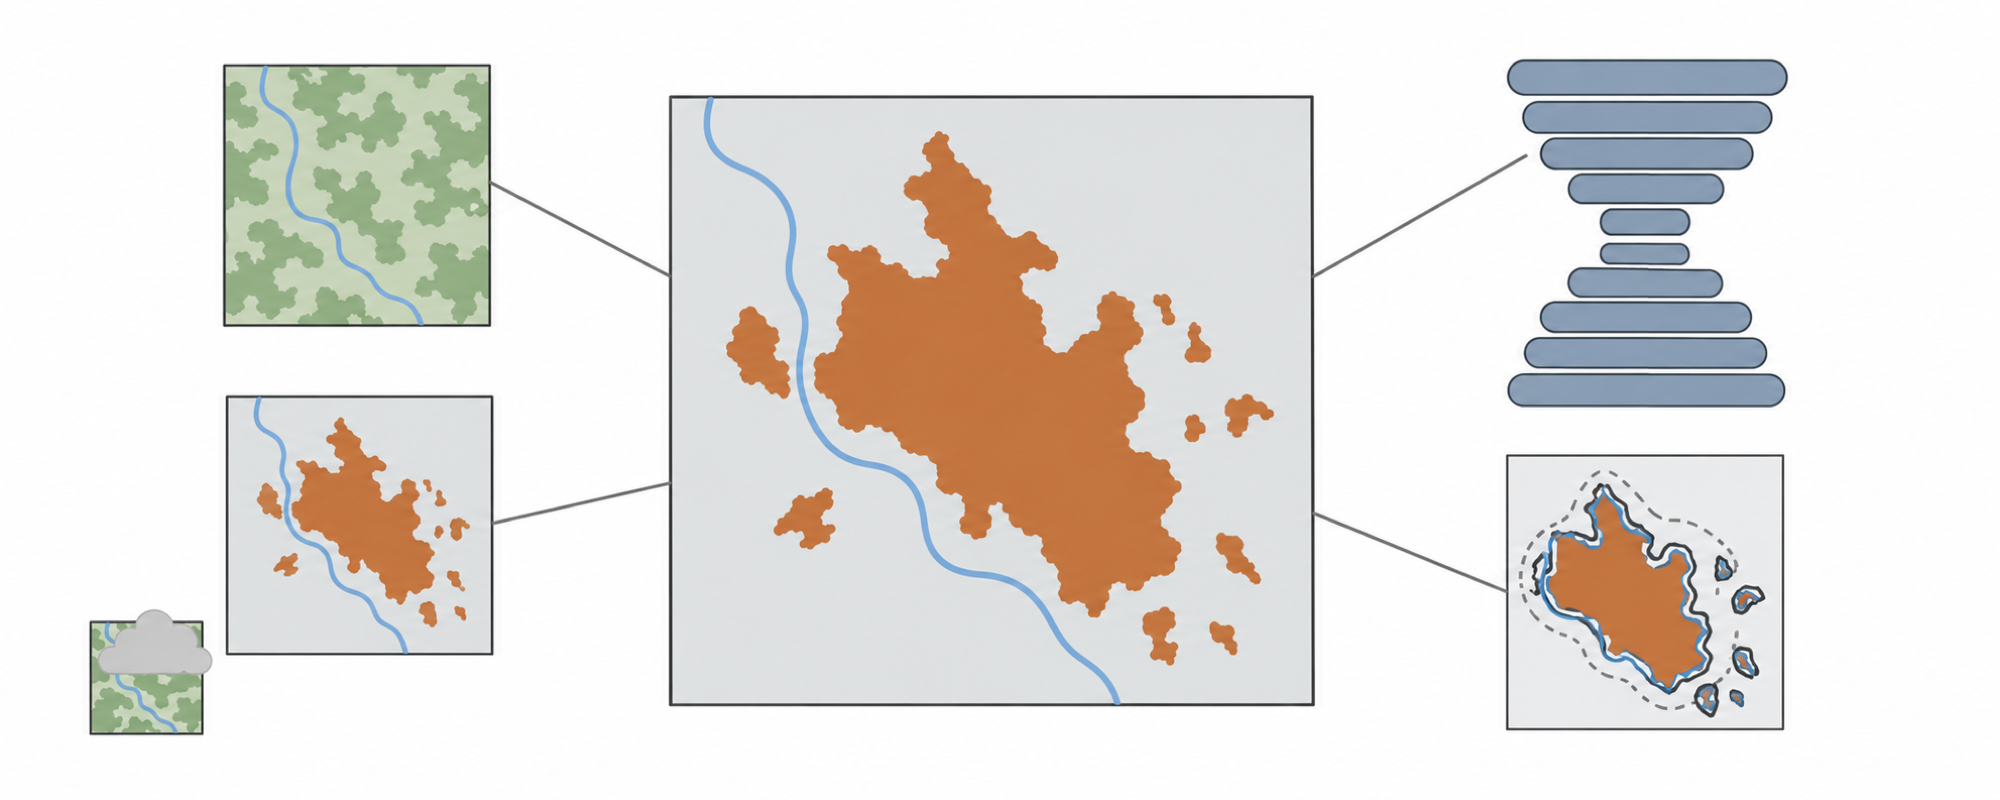
\includegraphics[width=\linewidth]{figures/ch10/ch10-04-composition-b-central.png}};
\begin{scope}[x={(img.south east)},y={(img.north west)}]
  \tikzset{stglbl/.style={font=\sffamily\scriptsize\bfseries,text=BookInk,fill=white,fill opacity=0.90,text opacity=1,inner sep=1.2pt,align=center}}
  \node[stglbl] at (0.175,0.54) {(1) 火前影像};
  \node[stglbl] at (0.175,0.11) {(1) 火后影像与云遮挡};
  \node[stglbl] at (0.82,0.45) {(2) 分割网络};
  \node[stglbl] at (0.49,0.05) {(3) 过火区图（中心）};
  \node[stglbl] at (0.82,0.04) {(4) 边界对比};
\end{scope}
\end{tikzpicture}
\caption{构图候选 B：中心图式。与图~\ref{fig:ch10-03} 内容相同。中心图吸引视线，但在 $5:2$ 横幅中，四周元素被压小，“比阈值法更贴近边界”的比较退到右下角落，在缩略图中最先看不清。\linebreak 若改投 $1200\ \text{px}$ 正方形格式，这种构图更容易适配。}\label{fig:ch10-04}
\end{figure}

观察图~\ref{fig:ch10-04} 也能看出中心图式在 $5:2$ 横幅中的局限：中央大图占了约 $77\%$ 的画布高度，四周元素被挤向左右两侧；右上角沙漏偏大，而右下角真正体现研究发现的边界对比插图被压得很小，内部细碎斑块与三条轮廓线在缩小时极易糊在一起；左下角的云遮挡小图块也退到了角落。表~\ref{tab:ch10-04-ab} 给出了两种构图的系统比较。

\begin{table}[htbp]\centering\footnotesize
\setlength{\tabcolsep}{3pt}
\renewcommand{\arraystretch}{1.15}
\caption{构图候选 A（左$\rightarrow$右叙事式）与候选 B（中心图式）的选型比较。}\label{tab:ch10-04-ab}
\begin{tabularx}{\linewidth}{@{}>{\raggedright\arraybackslash}p{24mm}YY@{}}
\toprule
\textbf{比较标准} & \textbf{候选 A：左$\rightarrow$右叙事式（图~\ref{fig:ch10-03}）} & \textbf{候选 B：中心图式（图~\ref{fig:ch10-04}）} \\
\midrule
阅读起点 & 唯一（最左侧火前/火后影像对） & 视线先落在中心大图，输入与对比分散在四周，起点不唯一 \\
终点是否为“发现” & 是（最右侧边界对比插图） & 中心图本身是“产出”，“优于阈值法”的对比被挤到右下角 \\
$5:2$ 横幅适配 & 好，四段横向展开，上下留出充足文字带 & 中心图高占约 $77\%$，上下难以排通栏文字，角落元素局促 \\
$200\ \text{px}$ 高缩略图 & 各阶段图标与主轮廓仍可辨 & 环绕的小元素与右下角细碎对比线在缩略图中最先消失 \\
限定条件位置 & 输入端上方云图标 + 底部通栏短句，读者顺路看到 & 云图标被挤到左下外角，易被忽略 \\
若改投 $1200\ \text{px}$ 正方形 & 需折成上下两行，阅读路径变 Z 字形 & 四角环绕中心大图的拓扑适配自然 \\
\midrule
\textbf{结论} & \textbf{选定 A}（本案例目标为 Elsevier 横幅） & {\raggedright 留作改投\newline 正方形格式时的备选} \\
\bottomrule
\end{tabularx}
\end{table}

两张候选图本身都干净整洁，最终选 A 而不是选 B，依据不是主观上的“哪张更好看”，而是画布长宽比、阅读起点与终点，以及限定条件在缩略图下的可见性。\linebreak
如果未来这篇论文改投要求提交 $1200 \times 1200\ \text{px}$ 正方形图形摘要的期刊，候选 B 的中心环绕布局反而更容易舒展。

\section{过度主张：当图像比论文说得更多}

假设合作者看了候选 A 后觉得“太素了，不够抢眼”，于是有人写了一句“让画面更震撼，突出 AI 的预警能力和全球意义”，提交了如下反例提示词：

\begin{Prompt}
Deliberately over-dramatic graphical abstract base art for a teaching
counter-example, wide banner, aspect ratio 5:2 (2000 x 800 px).
Dark blue gradient background with glowing accents.
Left: a photorealistic satellite-style top-down view of a forest with a bright
red-orange active fire front and thick gray smoke plumes.
Center: a glowing glossy 3D "AI brain" made of circuit lines, with light rays.
Right: a 3D Earth globe covered by a bright grid, with several red flame icons
on it, a red triangular alarm icon, and an alarm clock.
Glossy, cinematic, high contrast, lens flare.
NO TEXT: no letters, no words, no numbers, no symbols, no labels.
Leave a dark empty band across the top 18% for a headline.
\end{Prompt}

生成这张反例底图时有一个细节值得警惕：尽管提示词明确写了 \texttt{NO TEXT}，第 1 次生成仍在闹钟表盘上画出了 $1\text{--}12$ 数字并在红三角内画了感叹号，第 2 次生成在 12 点位置仍留下一条形似数字“1”的短刻线，直到第 3 次强制要求“空白表盘仅留两根指针、空心警报三角”才清掉所有内置字符。我们在第 3 次底图上用 TikZ 叠加上常见的夸大标题、百分比与预测口号（并附“虚构的夸大反例”水印防止截图误传），用红标 \textbf{O1—O7} 标出七处过度主张（图~\ref{fig:ch10-05}）。

\begin{figure}[htbp]\centering
\begin{tikzpicture}
\node[anchor=south west,inner sep=0] (img) at (0,0) {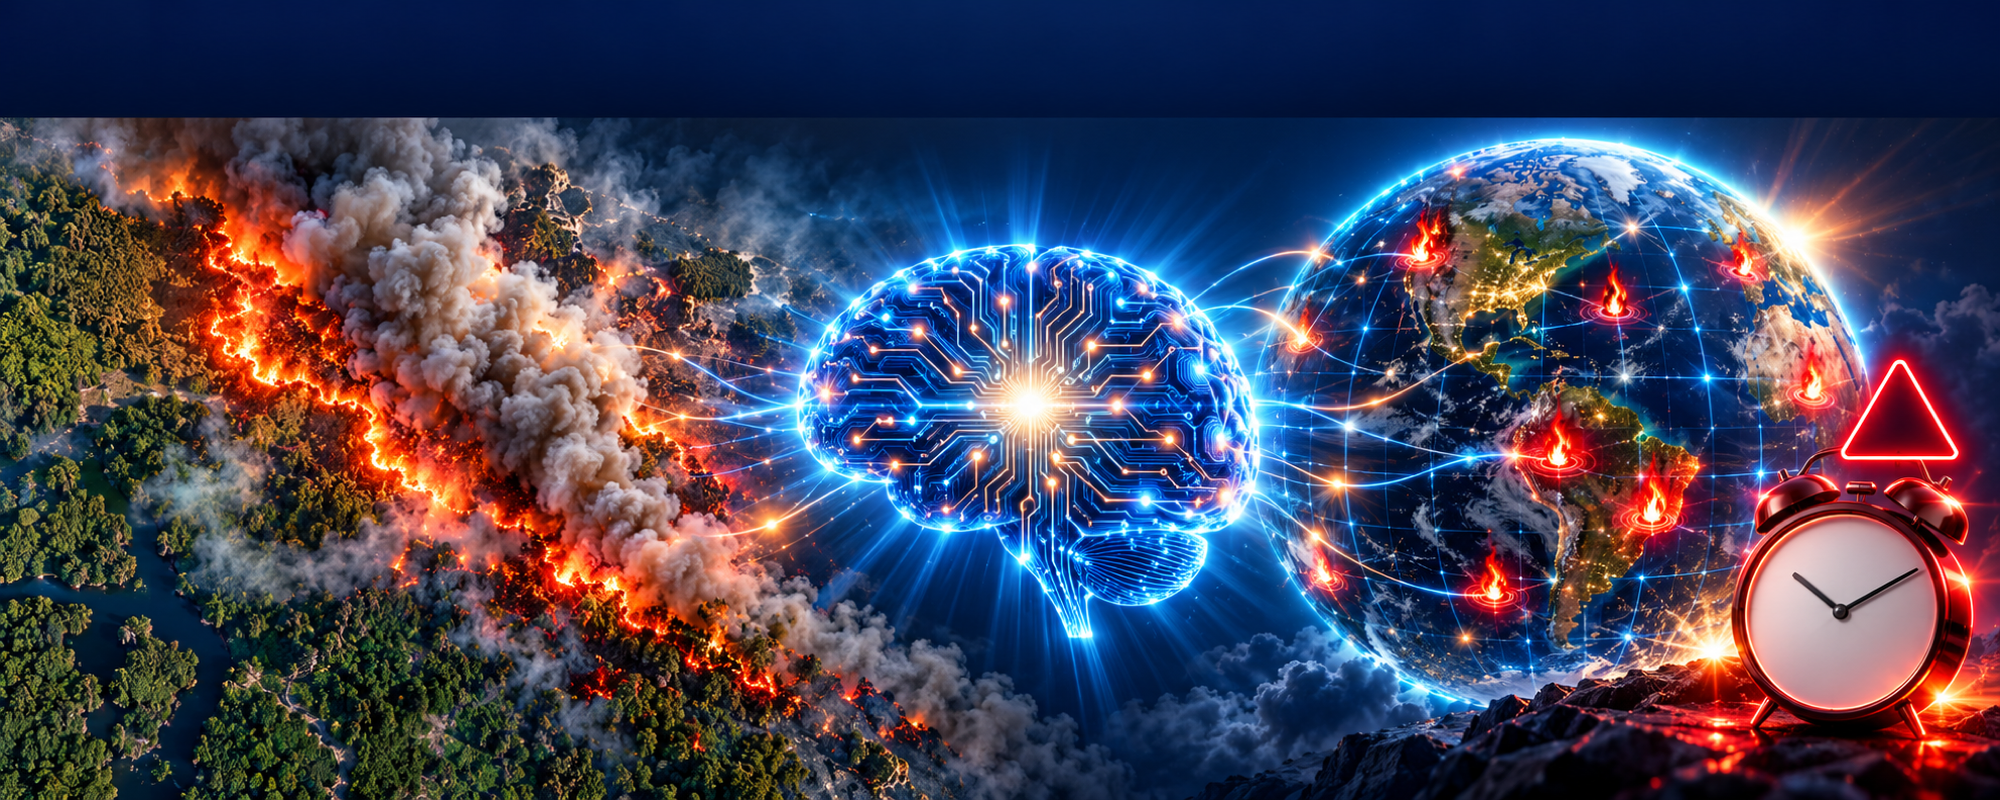
\includegraphics[width=\linewidth]{figures/ch10/ch10-05-overclaim.png}};
\begin{scope}[x={(img.south east)},y={(img.north west)}]
  \tikzset{
    overtxt/.style={font=\sffamily\bfseries,text=white,align=center},
    badmark/.style={draw=red!85!black,very thick,rounded corners=2pt,fill=white,fill opacity=0.92,text opacity=1,text=red!85!black,font=\sffamily\bfseries\scriptsize,inner sep=1.5pt}
  }
  \node[overtxt,font=\sffamily\normalsize\bfseries] at (0.52,0.92) {全球实时野火 AI（Real-time global wildfire AI）};
  \node[font=\sffamily\scriptsize\bfseries,text=yellow!90!white,fill=black!65,inner sep=1.5pt,rounded corners=1pt] at (0.50,0.81) {【虚构的夸大反例 · 非真实研究结果】};
  \node[overtxt,font=\sffamily\large\bfseries,text=yellow!95!white,fill=black!55,inner sep=2pt,rounded corners=2pt] at (0.50,0.45) {准确率 99\%};
  \node[overtxt,font=\sffamily\footnotesize\bfseries,fill=red!75!black,inner sep=2pt,rounded corners=2pt] at (0.72,0.12) {在起火前预测火灾};
  \node[badmark] at (0.09,0.34) {O1};
  \node[badmark] at (0.19,0.50) {O2};
  \node[badmark] at (0.77,0.56) {O3};
  \node[badmark] at (0.91,0.24) {O4};
  \node[badmark] at (0.37,0.45) {O5};
  \node[badmark] at (0.17,0.92) {O6};
  \node[badmark] at (0.27,0.70) {O7};
\end{scope}
\end{tikzpicture}
\caption{反例：过度主张的图形摘要（虚构示例）。照片质感的“卫星影像”、火线、地球、闹钟和无上下文的百分比，分别把“过火区制图”放大成观测证据、火点探测、全球覆盖、火灾预测和普适精度。图中的数字与标题均为故意夸大的虚构文字，不代表任何研究结果。底图由图像模型生成。}\label{fig:ch10-05}
\end{figure}

表~\ref{tab:ch10-05-overclaim} 逐项拆解了图~\ref{fig:ch10-05} 中 O1 至 O7 暗示的越界主张及保守修正方案。

\begin{table}[htbp]\centering\footnotesize
\setlength{\tabcolsep}{3pt}
\renewcommand{\arraystretch}{1.12}
\caption{图~\ref{fig:ch10-05} 中七处过度主张（O1--O7）的拆解与修正对照。}\label{tab:ch10-05-overclaim}
\begin{tabularx}{\linewidth}{@{}c>{\raggedright\arraybackslash}p{25mm}>{\raggedright\arraybackslash}p{25mm}>{\raggedright\arraybackslash}p{26mm}Y@{}}
\toprule
\textbf{\#} & \textbf{过度主张元素} & \textbf{它暗示了什么} & \textbf{论文实际支持什么} & \textbf{保守修正做法} \\
\midrule
O1 & 照片质感的森林俯视“影像” & 这是真实卫星观测照片 & 示意的火前/火后影像对；对象是已过火地表 & 改回扁平示意图块；图注说明“示意，非真实卫星影像” \\
O2 & 明亮火线、火焰图标与红色警报三角 & 活跃火点探测与应急报警 & 灾后已过火区域制图 & 删除火线、火焰与警报；过火区用暖棕橙色静态多边形 \\
O3 & 地球与覆盖全球的发光网格 & 全球各生态区通用 & 若干留出测试火场；跨生态区迁移未验证 & 删除地球与网格；只画单个示意地块并写明测试范围 \\
O4 & 闹钟与“在起火前预测火灾” & 能在起火前预测火灾发生 & 火后第一景无云影像到达后制图 & 删除闹钟与“预测”；改为“火后第一景无云影像即可绘制过火区” \\
O5 & 大号“准确率 99\%” & 有一个普适的高精度数字 & 仅报告比固定阈值基线更接近参考边界；数字需指标与对照 & 删除数字；用右侧三条边界线的贴合对比表达比较结论 \\
O6 & “全球实时野火 AI”标题 & 全球覆盖、实时响应 & 受重访周期与云烟限制 & 标题改为“火后第一景无云影像即可绘制过火区” \\
O7 & 浓烟滚滚却被 AI 光束直接穿透，且隐去无云限制 & 不受云烟遮挡、可全天候穿透观测 & 光学波段受云烟遮挡时一致性下降，依赖无云观测 & 删除穿透浓烟的光束；在输入端加回灰云遮挡图块与底部限定句 \\
\bottomrule
\end{tabularx}
\end{table}

特别注意 \textbf{O7}：画面左侧画了立体浓烟遮蔽森林，中央发光大脑的光束却直接穿透浓烟连向全球网格，同时把“需无云观测”的云朵图块删得一干二净，让人误以为光学波段能穿透浓烟作业。

\begin{BookNote}
\textbf{原则：图形摘要中的每一个图标都是一句陈述。}审稿人和读者会把“火焰”读作“探测火点”，把“地球”读作“全球通用”，把“闹钟”读作“事前预警”，把“穿透浓烟的光束”读作“不受云烟限制”。检查时把每个视觉元素翻译成一句陈述，再到论文里找它的依据，找不到就删。
\end{BookNote}

遇到图~\ref{fig:ch10-05} 这种整体跑偏的夸大稿，不要拿它当参考图局部修补，而应\textbf{直接退回候选 A 底图（图~\ref{fig:ch10-03}）}，下达如下精确微调指令：

\begin{Prompt}
以 A 稿为基础，不使用刚才的“震撼版”。保持 A 稿四段布局与所有对象不变。
不要火焰、烟柱、红色警报、地球、闹钟、照片质感影像，不要任何数字或文字。
只做两处修改：(1) 输出过火区图略放大约 1.2 倍；(2) 对比插图中三条边界线加粗，
使浅灰虚线与蓝色实线的偏离在缩小后仍可见。
\end{Prompt}

\section{定稿、缩略图测试与终稿核验}

我们按上述修改要求编写终稿英文提示词（完整版本见本书仓库 \texttt{cases/} 目录）：

\begin{Prompt}
Final graphical abstract base art, wide banner, aspect ratio 5:2,
2000 x 800 px, pure white background, flat 2D vector illustration, flat fills,
uniform thin dark gray (#3A3A3A) outlines, no gradients, no shadows, no 3D.
THIS IMAGE MUST CONTAIN NO TEXT AT ALL: no letters, words, numbers, symbols.
EMPTY BANDS: keep y 0.00-0.15 (top), y 0.76-0.84 (caption strip under the four
stages) and y 0.88-1.00 (bottom) completely white.
Four stages, all objects vertically within y 0.18-0.72:
1. x 0.04-0.25: two square schematic map tiles side by side (left: muted green
   #A8C3A0 vegetation; right: same patch with #C8743C burned area), same river.
   Smaller tile partly covered by a flat light gray (#D5D5D5) cloud at upper left.
2. x 0.30-0.45: one blue-gray (#8FA3B8) hourglass of stacked rounded rectangles.
3. x 0.50-0.73: one larger square map tile in very pale gray with a crisp
   #C8743C burned-area polygon (about 1.2 times the input tiles).
4. x 0.77-0.96: a square inset with three thick boundary lines: #3A3A3A solid
   (reference), #2F6DB5 solid closely following it, #A0A0A0 dashed deviating.
Two identical #3A3A3A arrows: stage 1 -> 2, stage 2 -> 3; no arrow between 3 and 4.
\end{Prompt}

终稿底图同样生成了三次：前两次未挂参考图独立生成时，第 1 次把沙漏网络画成了左右分开的 X 形双列且虚线偏离不够明显，第 2 次虽修好网络并加粗了边界线，但随机生成的河流与过火区形状与候选 A 不同；第 3 次\textbf{以候选 A（图~\ref{fig:ch10-03}）作为视觉参考图}生成，完整保留了候选 A 的河流走向、过火区轮廓、单列沙漏和两支流程箭头，同时将阶段 (4) 的三条对比边界线显著加粗。实测检查也记录下三处细微残余偏差：输出图块边长约为单块输入图块的 $1.6$ 倍（与左侧上下两层图块总高视觉齐平，而非严格 $1.2$ 倍）、部分图框下缘到约 $y=0.75$、留白带像素 RGB 在 $249\text{--}255$ 之间轻微浮动。这些几何与底色细节不影响科学表达，且三条文字空白带干净可用。

接着在无文字底图上用 TikZ 叠加七处矢量文字（表~\ref{tab:ch10-06-text}），得到图形摘要终稿（图~\ref{fig:ch10-06}）。

\begin{table}[htbp]\centering\footnotesize
\setlength{\tabcolsep}{3pt}
\renewcommand{\arraystretch}{1.15}
\caption{图形摘要终稿（图~\ref{fig:ch10-06}）叠加的矢量文字层（T1--T7）中英对照。}\label{tab:ch10-06-text}
\begin{tabularx}{\linewidth}{@{}cYY>{\raggedright\arraybackslash}p{28mm}@{}}
\toprule
\textbf{\#} & \textbf{中文文字层} & \textbf{英文文字层} & \textbf{位置与字号层级} \\
\midrule
T1 & 火后第一景无云影像即可绘制过火区 & Burned-area maps from the first clear post-fire image & $(0.50,0.07)$ 顶部居中；最大字号 \\
T2 & 火前 / 火后 Sentinel-2 影像对 & Pre-/post-fire Sentinel-2 pair & 阶段 (1) 下方；中号（缩略图可读） \\
T3 & 分割网络 & Segmentation network & 阶段 (2) 下方；中号（缩略图可读） \\
T4 & 过火区图 & Burned-area map & 阶段 (3) 下方；中号（缩略图可读） \\
T5 & 比 dNBR 阈值法更贴近参考边界 & Closer to reference edges than dNBR threshold & 阶段 (4) 下方；中号（缩略图可读） \\
T6 & 绘制已过火区域 · 非火点探测或预测 · 需无云观测 & Maps areas already burned $\cdot$ not fire detection or forecasting $\cdot$ needs cloud-free views & $(0.50,0.94)$ 底部居中；小号（文章页可读） \\
T7 & 参考 / 模型 / 阈值法 & reference / model / threshold & 对比插图下方小图例；最小字号 \\
\bottomrule
\end{tabularx}
\end{table}

\begin{figure}[htbp]\centering
\begin{tikzpicture}
\node[anchor=south west,inner sep=0] (img) at (0,0) {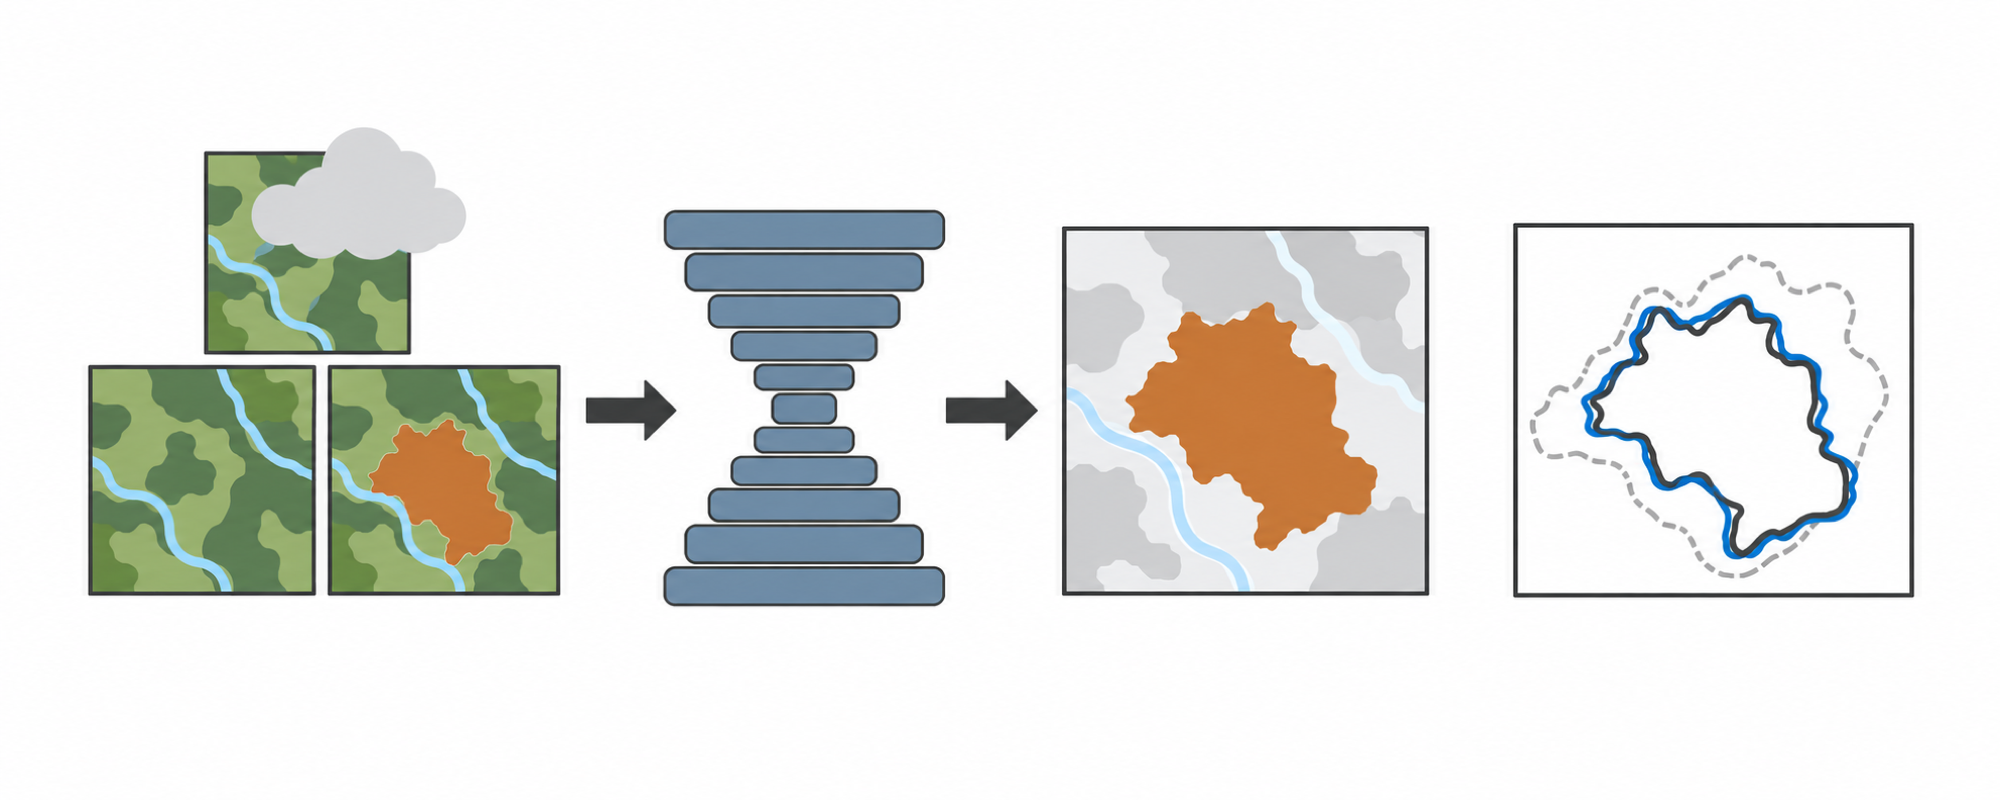
\includegraphics[width=\linewidth]{figures/ch10/ch10-06-final-base.png}};
\begin{scope}[x={(img.south east)},y={(img.north west)}]
  \tikzset{
    t1style/.style={font=\sffamily\small\bfseries,text=BookInk,align=center},
    tstg/.style={font=\sffamily\scriptsize\bfseries,text=BookInk,fill=white,fill opacity=0.90,text opacity=1,inner sep=1pt,align=center},
    t6style/.style={font=\sffamily\scriptsize,text=BookInk!90,align=center},
    t7style/.style={font=\sffamily\tiny,text=BookInk!85,align=center}
  }
  \node[t1style] at (0.50,0.92) {火后第一景无云影像即可绘制过火区};
  \node[tstg] at (0.165,0.18) {火前 / 火后 Sentinel-2 影像对};
  \node[tstg] at (0.40,0.18) {分割网络};
  \node[tstg] at (0.62,0.18) {过火区图};
  \node[tstg] at (0.855,0.18) {比 dNBR 阈值法更贴近参考边界};
  \node[t7style] at (0.855,0.11) {参考 / 模型 / 阈值法};
  \node[t6style] at (0.50,0.04) {绘制已过火区域 · 非火点探测或预测 · 需无云观测};
\end{scope}
\end{tikzpicture}
\caption{教学案例的图形摘要终稿。左$\rightarrow$右依次为火前/火后影像对、分割网络、过火区图，以及与参考边界的比较示意。底部一句写明限定条件。全部影像均为扁平示意图块，\textbf{非真实卫星影像}；研究情境为本章虚构的教学案例，不对应已发表结果。底图由图像模型生成，文字以 TikZ 叠加。}\label{fig:ch10-06}
\end{figure}

最后一步是把“缩到目录尺寸还看得清吗”变成可重复的\textbf{缩略图测试（thumbnail test）}。当 $2000 \times 800\ \text{px}$ 的原图被缩放到 Elsevier 指南所述的 $200\ \text{px}$ 高目录窗口（即 $500 \times 200\ \text{px}$）时，线性尺寸缩小为原来的四分之一。若原图阶段名采用约 $36\ \text{px}$ 字高，缩后约为 $9.0\ \text{px}$ 高，仍可辨认；若原图只用 $14\ \text{px}$ 字高，缩后仅剩约 $3.5\ \text{px}$ 高，笔画彻底糊成一团（图~\ref{fig:ch10-07}）。同时注意，关键限定条件必须像 T6 这样写在图内（配合左上角云图标），不能只写在图外图注里。

\begin{figure}[htbp]\centering
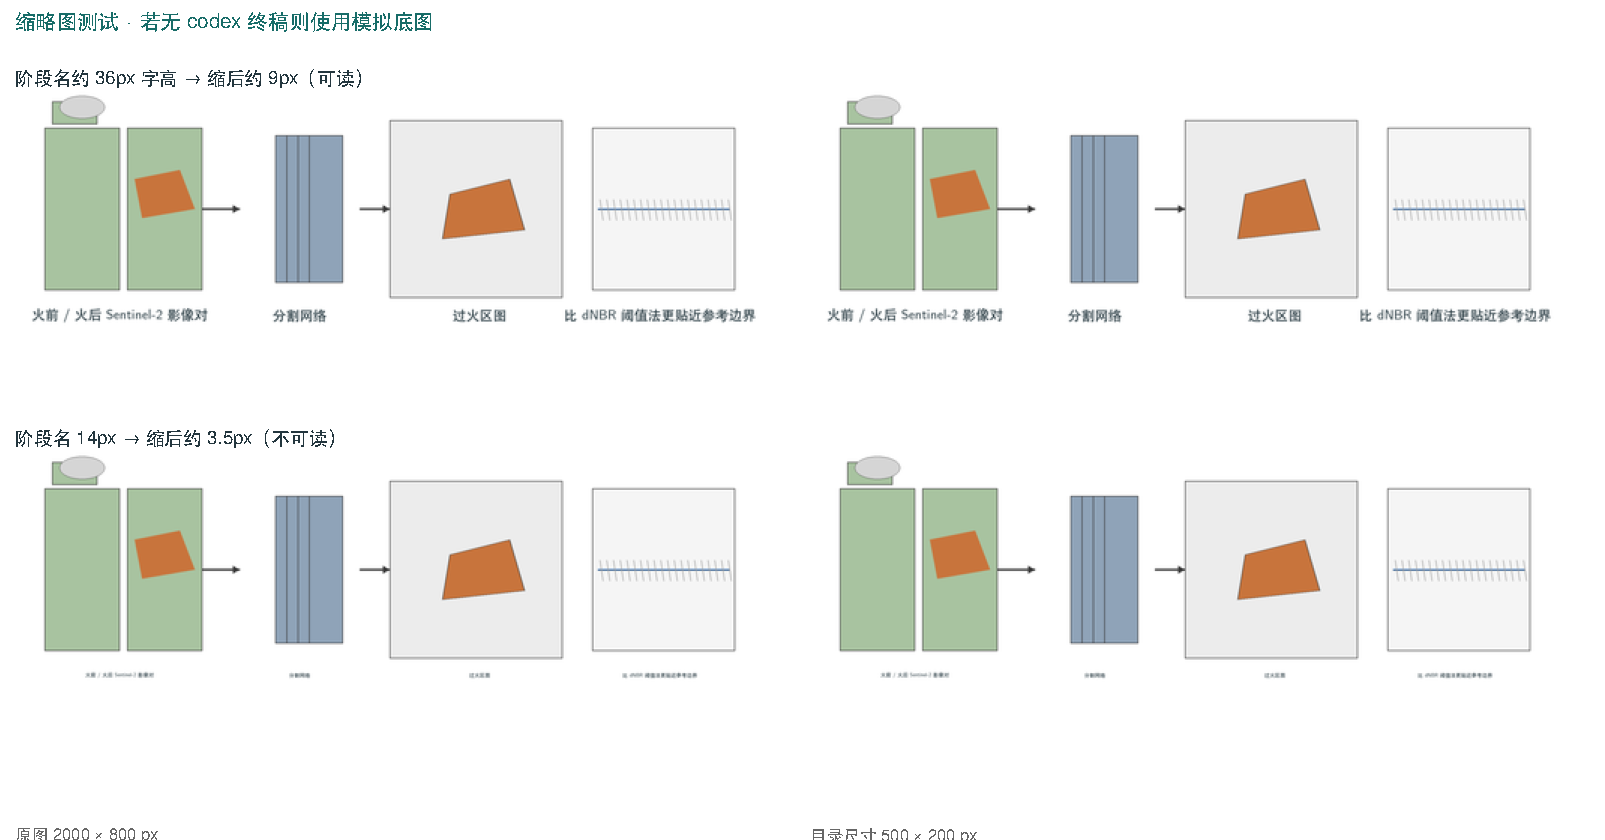
\includegraphics[width=\linewidth]{figures/ch10/ch10-07-thumbnail-test-zh.pdf}
\caption{缩略图测试。把图形摘要缩到约 $200\ \text{px}$ 高（Elsevier 指南所述的目录显示高度）后，以实际像素显示（本图在相同 $2000 \times 800\ \text{px}$ 模拟布局底图上仅改变阶段名字高进行对照）。上：阶段名约 $36\ \text{px}$ 字高，缩后约 $9\ \text{px}$ 高，仍可辨认；下：同一张图只把阶段名改小为 $14\ \text{px}$，缩小后约 $3.5\ \text{px}$ 高，已无法阅读。底部限定句在缩略图中较小，但在文章页中可读。}\label{fig:ch10-07}
\end{figure}

\section{本章完整案例回顾与核验表}

回顾本案例，我们从一篇虚构教学摘要出发，依次完成了期刊规格核查（图~\ref{fig:ch10-01}）、四行贡献卡提炼（表~\ref{tab:ch10-02-card}）、PDF 转提示词边界比对（图~\ref{fig:ch10-02}、表~\ref{tab:ch10-03-compare}）、A/B 两种构图比选（图~\ref{fig:ch10-03}、图~\ref{fig:ch10-04}、表~\ref{tab:ch10-04-ab}）、过度主张反例拆解（图~\ref{fig:ch10-05}、表~\ref{tab:ch10-05-overclaim}）、终稿底图修改与矢量叠字（图~\ref{fig:ch10-06}），以及 $200\ \text{px}$ 高缩略图实测（图~\ref{fig:ch10-07}）。终稿交付前的九项核验记录汇总于表~\ref{tab:ch10-07-verify}。

\begin{table}[htbp]\centering\footnotesize
\setlength{\tabcolsep}{3pt}
\renewcommand{\arraystretch}{1.15}
\caption{教学案例图形摘要终稿（图~\ref{fig:ch10-06}）的九项核验表（C1--C9）。}\label{tab:ch10-07-verify}
\begin{tabularx}{\linewidth}{@{}c>{\raggedright\arraybackslash}p{26mm}>{\raggedright\arraybackslash}p{32mm}Y@{}}
\toprule
\textbf{\#} & \textbf{检查项} & \textbf{核验方法} & \textbf{结果记录} \\
\midrule
C1 & 贡献卡四行都在图中 & 逐行指出对应元素 & 问题与方法对应阶段 (1)--(3) 及 T1--T4；发现对应阶段 (4) 与 T5；限定对应左上灰云图块与底部 T6 短句 \\
C2 & 无超出论文的元素 & 把每个图标翻译成一句话并在摘要中找依据 & 全部对象均为任务书规定的示意元素，无火焰、地球、闹钟或百分比数字 \\
C3 & 无数字、无数据图、无照片质感影像 & 放大检查纹理与图形类别 & 无数字与数据图；影像为扁平示意图块（填色带轻微明暗变化，图注已标明非真实卫星影像） \\
C4 & 比例与像素 & 检查文件属性：$5:2$，$\ge 1328 \times 531\ \text{px}$ & 交付底图为 $2000 \times 800\ \text{px}$，满足 $5:2$ 比例与像素要求 \\
C5 & 缩略图可读 & 图~\ref{fig:ch10-07} 测试：$200\ \text{px}$ 高下阶段名可读 & 阶段名按约 $36\ \text{px}$ 字高设置，缩至 $200\ \text{px}$ 高后约 $9\ \text{px}$ 高，可辨认 \\
C6 & 底图无伪文字 & 原尺寸放大检查 & 选定底图未见字母、数字或伪文字（反例图前两次出现的表盘数字与刻线已淘汰重出） \\
C7 & 中英两版只有文字层不同 & 比对底图文件哈希值 & 中英两版共用同一无字底图文件，仅 TikZ 叠加文字层按表~\ref{tab:ch10-06-text} 切换 \\
C8 & 期刊要求已在提交前复核 & 记录目标期刊页面 URL 与访问日期 & 已记录 Elsevier 通用指南 URL 与 2026 年 10 月访问日期；投具体子刊前须再次复核 \\
C9 & PDF 转提示词的读取范围与原文已存档 & 检查本地图片档案记录 & 使用 \sdtool{graphical-abstract-maker} 时，将前 5 页读取范围、返回提示词原文与比对表一并存档 \\
\bottomrule
\end{tabularx}
\end{table}

\section{AI 在这一步能做什么与不能做什么}

图形摘要制作各环节中 AI 与作者的职责边界汇总于表~\ref{tab:ch10-08-ai}。

\begin{table}[htbp]\centering\footnotesize
\setlength{\tabcolsep}{3pt}
\renewcommand{\arraystretch}{1.15}
\caption{图形摘要制作环节中 AI 能做什么、不能做什么与作者要核对的内容。}\label{tab:ch10-08-ai}
\begin{tabularx}{\linewidth}{@{}>{\raggedright\arraybackslash}p{16mm}YYY@{}}
\toprule
\textbf{环节} & \textbf{AI（\scidraw{} 等）能做} & \textbf{AI 不能做} & \textbf{作者要核对} \\
\midrule
读论文 & 图形摘要入口读取 PDF 前 5 页（约 $6{,}000$ 字符以内），生成 $60\text{--}110$ 词视觉提示词 & 理解全文；判断哪个发现最重要；保证保留限定条件 & 记录读取范围与输出原文；与贡献卡逐行比对，补回限定条件 \\
提炼贡献 & 帮你把摘要改写成更短的句子；列出可能的视觉对象 & 决定论文的核心贡献；判断措辞强度是否与证据相符 & 每一行能否在论文中找到原句；“优于”“解决”“预测”等词是否越界 \\
构图 & 按提示词生成同一构图的多个候选；按要求生成第二种构图 & 自动提出“有理由的”不同构图并解释取舍（批量候选只是随机变体） & 两种构图分别写明；用比例、阅读路径、缩略图、限定条件可见性比较 \\
生成底图 & 扁平示意风格、无字底图、留白区域（结果有随机性） & 保证无伪文字；精确位置；保证示意影像不被读成真实观测 & 放大查伪文字；影像必须是示意风格并在说明中注明 \\
修改 & 以历史图为参考图按指令修改 & 对象锁定；保证只改指定处 & 每次修改后重做整张核验（见第 11 章） \\
文字 & （不建议）在图中生成文字 & 可靠拼写与对位 & 文字用 TikZ 或排版软件叠加；逐字比对 \\
交付 & 导出图片 & 判断目标期刊当前要求 & 打开目标期刊页面核对比例、像素、字体、格式并记录日期；缩略图测试 \\
诚信 & — & 判断某个图标是否构成过度主张 & 把每个元素翻译成一句陈述，在论文中找依据 \\
\bottomrule
\end{tabularx}
\end{table}

\section{本章检查清单}

\begin{itemize}
\item 已打开目标期刊\textbf{当前}的图形摘要要求页面，记录了 URL、访问日期、比例、像素、字体与格式。
\item 贡献卡四行（问题 / 方法 / 发现 / 限定）都能在论文中找到原句，措辞强度没有升级。
\item 若使用了 PDF 转提示词：已存档读取范围（前 5 页）与输出原文，并逐行比对、补回限定条件。
\item 至少有两种\textbf{写明理由}的构图候选，并按比例、阅读起点与终点、缩略图可读性、限定条件位置选定。
\item 图中每个图标都能翻译成论文支持的一句话；没有火焰、地球、闹钟、数字一类“替你多说话”的元素，除非论文确实支持。
\item 示意影像不是照片质感；如使用真实影像，来源、许可与处理已写明。
\item 底图无伪文字；文字全部叠加并逐字核对；总字数克制。
\item 缩到目录尺寸（如 $200\ \text{px}$ 高）后阶段名仍可读，阅读路径清楚。
\item 中英两版只在文字层不同。
\item 档案中记录了工具、提示词、生成次数和人工修改。
\end{itemize}

\section{练习}

\begin{enumerate}
\item \textbf{（贡献卡：纸笔练习）}选一篇你所在领域近期的论文，只读摘要和结论，写出四行贡献卡；再通读结果部分，修改“发现”与“限定”两行。比较两次的差别，并说明哪一处措辞如果写进图形摘要会构成过度主张。
\item \textbf{（\scidraw{} 实操：PDF 转提示词的比对）}打开 \scidraw{} 的图形摘要工具 \sdtool{graphical-abstract-maker}，上传你自己（或练习 1）的论文 PDF，保存返回的视觉提示词。做一张比对表：贡献卡每一行在提示词中是“保留”“丢失”还是“被加强”。据此写出修改后的生成提示词，生成一版候选，并完成本章检查清单。
\item \textbf{（改格式）}把本章终稿（$5:2$）改成 $1200 \times 1200\ \text{px}$ 正方形的方案：画出草图，说明你会改用候选 A 的两行折叠还是候选 B 的中心图式、限定条件放在哪里，以及缩略图测试应怎样调整。
\end{enumerate}

\section*{参考文献}

\begin{itemize}
\item American Chemical Society. \textit{The Journal of Organic Chemistry} Author Guidelines. \url{https://researcher-resources.acs.org/publish/author_guidelines?coden=joceah} (accessed 2026-10-29).
\item American Chemical Society. \textit{Langmuir} Author Checklist. \url{https://pubs.acs.org/page/langd5/submission/author-checklist} (accessed 2026-10-29).
\item Cell Press. Attract readers at a glance with your Graphical Abstract. \url{https://crosstalk.cell.com/blog/attract-readers-at-a-glance-with-your-graphical-abstract} (accessed 2026-10-29).
\item Cell Press. \textit{Cell Reports} Final File Requirements. \url{https://www.cell.com/pb-assets/journals/EM/MasterFFCs/CELREPFFC-1750868285900.pdf} (accessed 2026-10-29).
\item Chuvieco E, Mouillot F, van der Werf GR, et al. Historical background and current developments for mapping burned area from satellite Earth observation. \textit{Remote Sensing of Environment}. 2019;225:45--64. \url{https://doi.org/10.1016/j.rse.2019.02.013}
\item Elsevier. Graphical abstracts — Author tools and resources. \url{https://www.elsevier.com/researcher/author/tools-and-resources/graphical-abstract} (accessed 2026-10-29).
\item Giglio L, Boschetti L, Roy DP, Humber ML, Justice CO. The Collection 6 MODIS burned area mapping algorithm and product. \textit{Remote Sensing of Environment}. 2018;217:72--85. \url{https://doi.org/10.1016/j.rse.2018.08.005}
\item Ibrahim AM, Lillemoe KD, Klingensmith ME, Dimick JB. Visual abstracts to disseminate research on social media: a prospective, case-control crossover study. \textit{Annals of Surgery}. 2017;266(6):e46--e48. \url{https://doi.org/10.1097/SLA.0000000000002277}
\item Knopp L, Wieland M, Rättich M, Martinis S. A deep learning approach for burned area segmentation with Sentinel-2 data. \textit{Remote Sensing}. 2020;12(15):2422. \url{https://doi.org/10.3390/rs12152422}
\item Pferschy-Wenzig E-M, Pferschy U, Wang D, Mocan A, Atanasov AG. Does a graphical abstract bring more visibility to your paper? \textit{Molecules}. 2016;21(9):1247. \url{https://doi.org/10.3390/molecules21091247}
\item Roy DP, Huang H, Boschetti L, et al. Landsat-8 and Sentinel-2 burned area mapping — a combined sensor multi-temporal change detection approach. \textit{Remote Sensing of Environment}. 2019;231:111254. \url{https://doi.org/10.1016/j.rse.2019.111254}
\end{itemize}

% TODO: 1) SciDraw AI `/zh/graphical-abstract-maker` 上传 `teaching-paper.pdf` 的在线实测返回提示词（`provenance/ch10/pdf-prompt.txt`）待补测归档；
% TODO: 2) `figures/ch10/ch10-07-thumbnail-test-zh.pdf` 当前使用脚本内置的模拟底图（`simulated_base: true`），待接入 `ch10-06-final-base.png` 合成终稿后重新生成；
% TODO: 3) Cell Press 总指南页（`https://www.cell.com/figureguidelines`）此前被访问验证拦截，以及 ACS 通用图形指南“字号不小于 8 pt”条款，待人工打开原始页面复核。
